\documentclass[tikz,border=8pt]{standalone}
% Shared look for every TikZ diagram. Load with \input{../../tools/tikz-style.tex}
\usepackage[T1]{fontenc}
\usepackage{lmodern}
\renewcommand{\sfdefault}{lmr}  % diagrams use the same serif as the text
\usetikzlibrary{arrows.meta, positioning, shapes.geometric, calc, fit, backgrounds}
\definecolor{cblue}{HTML}{4C78A8}
\definecolor{corange}{HTML}{F58518}
\definecolor{cgreen}{HTML}{54A24B}
\definecolor{cred}{HTML}{E45756}
\definecolor{cpurple}{HTML}{B279A2}
\definecolor{cgrey}{HTML}{6B6B6B}
\tikzset{
  every picture/.style={font=\sffamily, line width=1.2pt},
  box/.style={draw=#1, fill=#1!12, rounded corners=4pt, align=center, inner sep=7pt, minimum height=1.1cm},
  box/.default=cgrey,
  arrow/.style={-{Stealth[length=3mm]}, draw=cgrey, line width=1.4pt},
  title/.style={font=\sffamily\bfseries\Large},
  note/.style={font=\sffamily\small, text=cgrey, align=center},
}
\AtBeginDocument{\hyphenpenalty=10000 \exhyphenpenalty=10000}

\usepackage{textcomp}
\begin{document}
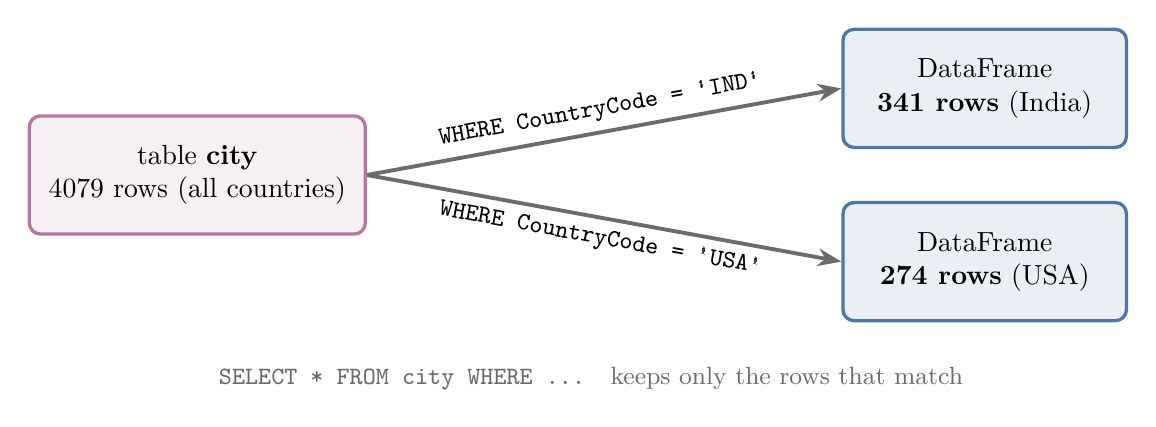
\begin{tikzpicture}
  \tikzset{tb/.style={box=#1, minimum width=3.6cm, minimum height=1.5cm}}
  \node[tb=cpurple] (all) at (0,0) {table \textbf{city}\\4079 rows (all countries)};
  \node[tb=cblue] (ind) at (10,1.1)  {DataFrame\\\textbf{341 rows} (India)};
  \node[tb=cblue] (usa) at (10,-1.1) {DataFrame\\\textbf{274 rows} (USA)};
  \draw[arrow] (all.east) -- node[above, sloped, font=\ttfamily\small]{WHERE CountryCode = \textquotesingle IND\textquotesingle} (ind.west);
  \draw[arrow] (all.east) -- node[below, sloped, font=\ttfamily\small]{WHERE CountryCode = \textquotesingle USA\textquotesingle} (usa.west);
  \node[note, anchor=north] at (5,-2.3) {\texttt{SELECT * FROM city WHERE ...}\quad keeps only the rows that match};
\end{tikzpicture}
\end{document}
